\documentclass[a4paper,oneside,10pt]{article}
\usepackage{wallpaper}
\usepackage{float}
\usepackage[utf8]{inputenc}
\usepackage[T1]{fontenc}
\usepackage[brazil]{babel}
\usepackage{circuitikz}
\usepackage{amsmath}
\usepackage{listings}
\usepackage{xcolor}
\usepackage{hyperref}
\usepackage{indentfirst}

\setlength{\textwidth}{16cm} %
\setlength{\textheight}{23cm} %
\setlength{\oddsidemargin}{0cm} %
\setlength{\evensidemargin}{0cm} %
\setlength{\topmargin}{0cm}

\CenterWallPaper{1.01}{bg.pdf}

% Configuração visual para o bloco de código Arduino/C++
\definecolor{codegreen}{rgb}{0,0.6,0}
\definecolor{codegray}{rgb}{0.5,0.5,0.5}
\definecolor{codepurple}{rgb}{0.58,0,0.82}
\definecolor{backcolour}{rgb}{0.96,0.96,0.96}

\lstdefinestyle{arduinoStyle}{
    backgroundcolor=\color{backcolour},   
    commentstyle=\color{codegreen},
    keywordstyle=\color{blue}\bfseries,
    numberstyle=\tiny\color{codegray},
    stringstyle=\color{codepurple},
    basicstyle=\ttfamily\footnotesize,
    breakatwhitespace=false,         
    breaklines=true,                 
    captionpos=b,                    
    keepspaces=true,                 
    numbers=left,                    
    numbersep=5pt,                  
    showspaces=false,                
    showstringspaces=false,
    showtabs=false,                  
    tabsize=2,
    language=C++,
    literate={á}{{\'a}}1 {ã}{{\~a}}1 {é}{{\'e}}1 {ê}{{\^e}}1 {í}{{\'i}}1 {ó}{{\'o}}1 {õ}{{\~o}}1 {ú}{{\'u}}1 {ç}{{\c{c}}}1 {Á}{{\'A}}1
}

\lstset{style=arduinoStyle}

\begin{document}

\noindent Relatório 8: Conectividade Wi-Fi. \\
Internet das Coisas Integral\\
Prof. Gabriel de Freitas Fernandes\\
2026.2\\
\\
\textbf{EQUIPE:} \\ Arthur Peixoto - 170.214 \\ Gabriel Oliva Gurgel - 168.860 \\ Guilherme Samuel dos Santos - 168.867

\section{Introdução}
Esta prática tem como objetivo implementar a conexão de um microcontrolador ESP32 à rede Wi-Fi para enviar dados de sensores e atuadores diretamente para uma planilha no Google Drive. No contexto de Internet das Coisas (IoT), essa integração é fundamental para monitorar informações de forma remota e automática. 

Para atingir esse objetivo, utilizaram-se as bibliotecas de rede do ESP32 e uma ferramenta de integração com o Google Sheets. O sistema foi programado para escanear as redes Wi-Fi disponíveis, exibir a intensidade do sinal de cada uma, permitir a conexão interativa via terminal e registrar os dados coletados de forma periódica na planilha.

\section{Prática}

\subsection{Montagem Experimental}
O esquema eletrônico seguiu o mesmo que o estabelecido anteriormente com o módulo conversor analógico-digital externo \textbf{ADS1115}, um sensor LDR simples e um servomotor \textbf{MG996R}.

\begin{figure}[H]
	\centering
	\begin{minipage}[b]{0.5\textwidth}
		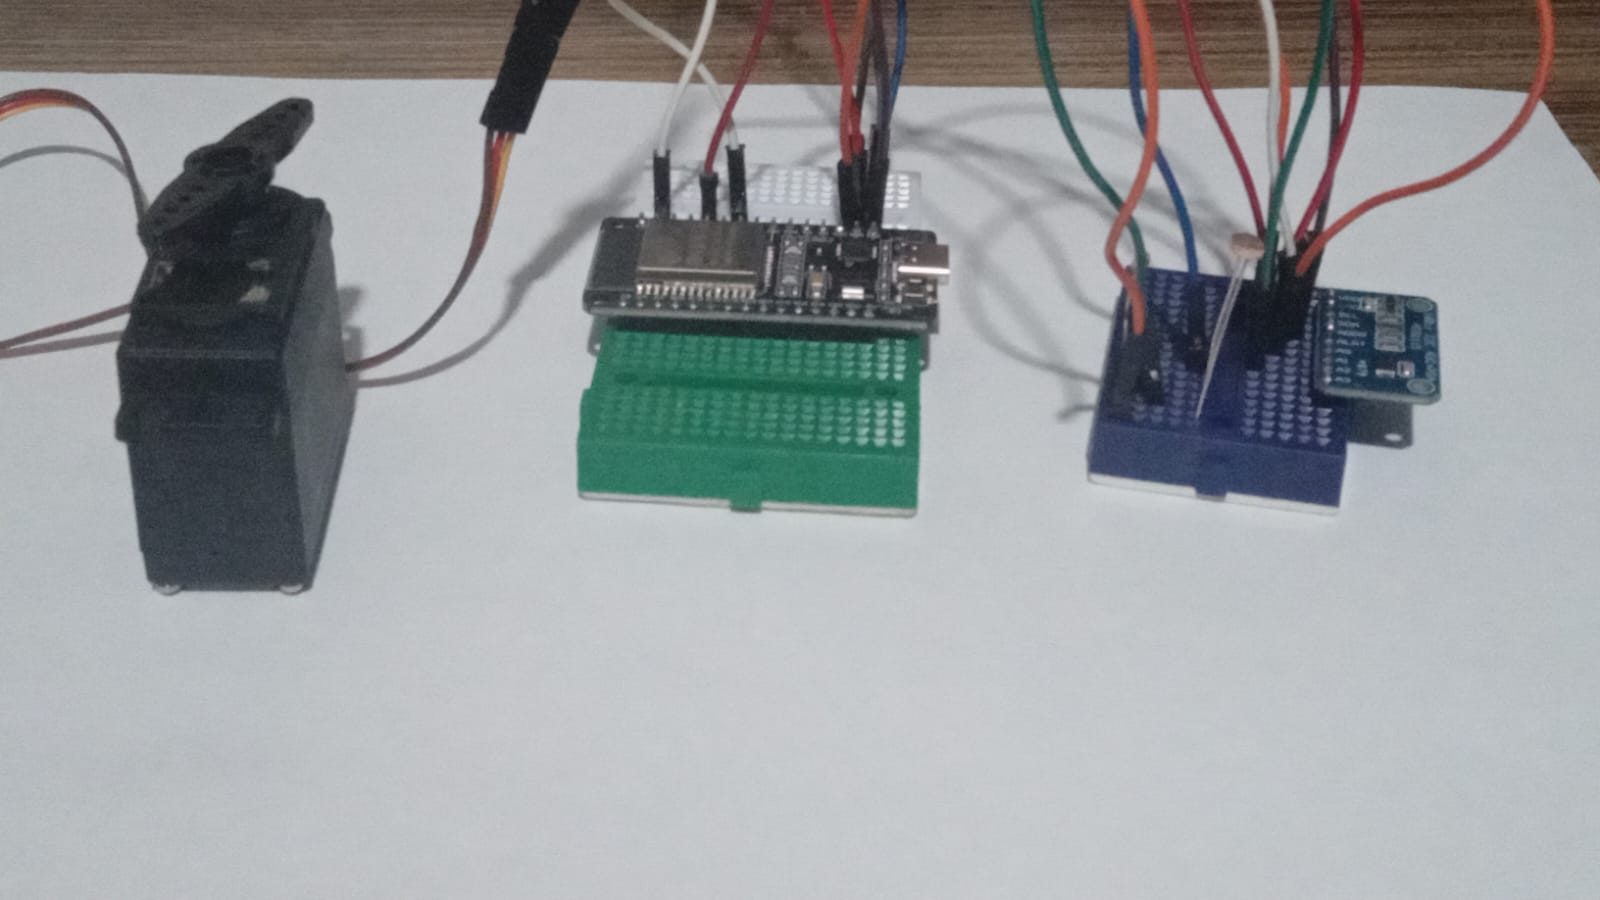
\includegraphics[width=\textwidth]{v1}
		\caption{Versão feita de teste no pós-aula (sem capacitor)}
	\end{minipage}
	\hfill
	\begin{minipage}[b]{0.45\textwidth}
		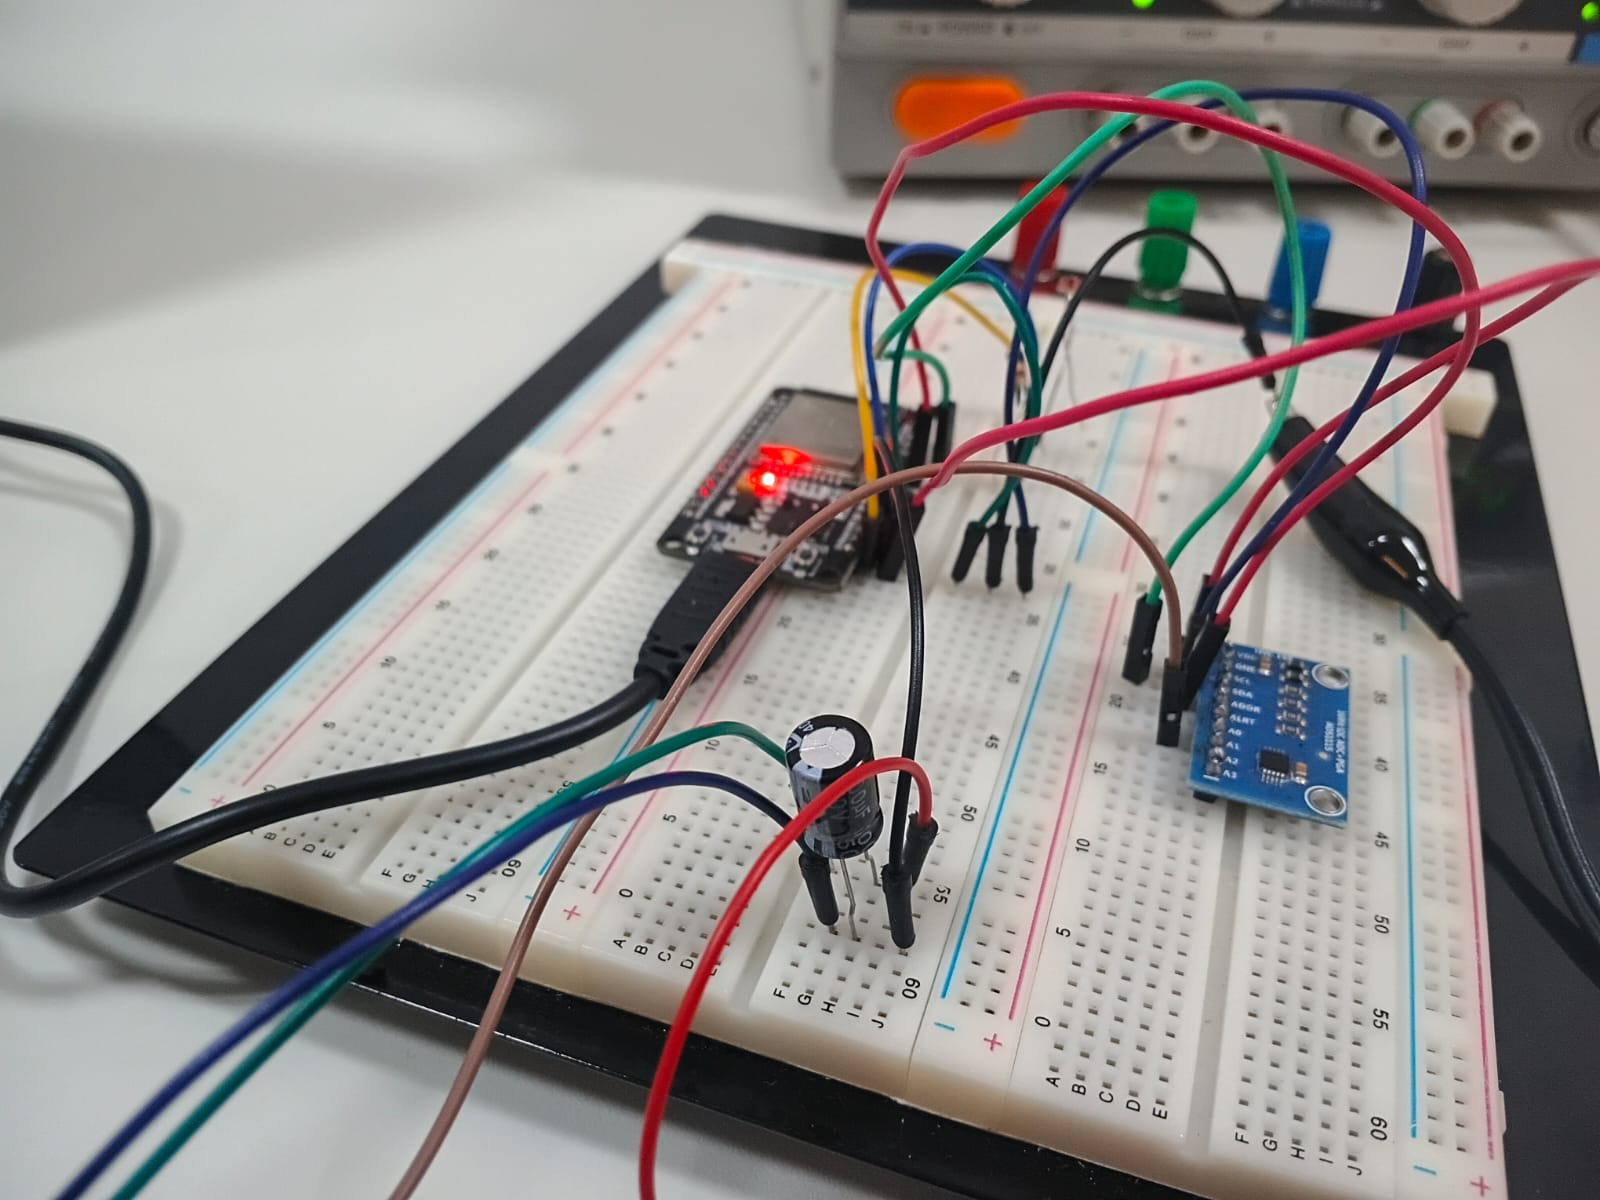
\includegraphics[width=\textwidth]{v2}
		\caption{Versão feita de teste durante aula
			(com capacitor)}
	\end{minipage}
\end{figure}

\subsection{Código}

O código desenvolvido na Arduino IDE para estabelecer a conectividade Wi-Fi e sincronizar os dados com a planilha eletrônica é apresentado na Listagem \ref{lst:wifi_code}. As variáveis \texttt{dado1} e \texttt{dado2} representam os canais de dados utilizados para o envio.

Para questões de simplificação, a chave privada foi reduzida a uma \textit{string} simples no exemplo a seguir. Ela está presente na versão de anexo.

\newpage

\begin{lstlisting}[caption={Implementação da varredura Wi-Fi e envio de dados para o Google Sheets no ESP32.}, label={lst:wifi_code}]
#include <WiFi.h>
#include <ESP_Google_Sheet_Client.h>
#include <ESP32Servo.h>
#include <Adafruit_ADS1X15.h>
#include <Wire.h>

Adafruit_ADS1115 ads;
Servo servo;

#define MOTOR_PIN 18
#define PROJECT_ID "projeto-do-dragao-guerreiro"
#define CLIENT_EMAIL "esp32iot@projeto-do-dragao-guerreiro.iam.gserviceaccount.com"
#define SPREADSHEET_ID "1dnOn1AiQJhA3T02qwPbDCbBpHlYDftc1H0ZB63vDMWQ"
const char PRIVATE_KEY[] PROGMEM = "my-private-key";

bool leituraConcluida = false;
bool gsheetInitialized = false;

unsigned long ultimoEnvio = 0;
const unsigned long intervaloEnvio = 5000; // Intervalo de 5 segundos entre envios

// 3 variáveis com valores 1, 2 e 3
int dado1 = 1;
int dado2 = 2;
int dado3 = 3;

String ssid = "";
String password = "";

String readSerialLine() {
	while (Serial.available() == 0) {
		delay(50);
	}
	String input = Serial.readStringUntil('\n');
	input.trim();
	return input;
}

void conectarWifiPelaSerial() {
	while (WiFi.status() != WL_CONNECTED) {
		Serial.println("\n--- Internet Scan ---");
		int n = WiFi.scanNetworks();
		
		if (n == 0) {
			Serial.println("Nenhuma rede detectada.");
			delay(3000);
			continue;
		}
		
		Serial.print("Foram encontradas ");
		Serial.print(n);
		Serial.println(" redes:");
		for (int i = 0; i < n; ++i) {
			Serial.print(i + 1);
			Serial.print(": ");
			Serial.print(WiFi.SSID(i));
			Serial.print(" (");
			Serial.print(WiFi.RSSI(i));
			Serial.print(" dBm)");
			Serial.println((WiFi.encryptionType(i) == WIFI_AUTH_OPEN) ? " [Open]" : " [Locked]");
			delay(10);
		}
		
		// Limpa caracteres residuais no buffer da serial
		while (Serial.available() > 0) {
			Serial.read();
		}
		
		Serial.println("\nQual o nome (SSID) da rede que pretende conectar?");
		ssid = readSerialLine();
		Serial.println("Rede selecionada: " + ssid);
		
		Serial.println("Qual a senha dessa rede? Se for pública digite 0:");
		password = readSerialLine();
		
		Serial.print("A conectar a " + ssid);
		if (password == "0" || password.length() == 0) {
			WiFi.begin(ssid.c_str());
		} else WiFi.begin(ssid.c_str(), password.c_str());
		
		int t = 0;
		while (WiFi.status() != WL_CONNECTED && t < 20) {
			Serial.print(".");
			delay(500);
			t++;
		}
		
		if (WiFi.status() == WL_CONNECTED) {
			Serial.println("\nConectado ao Wi-Fi com sucesso!");
			Serial.print("IP ESP32: ");
			Serial.println(WiFi.localIP());
			Serial.print("RSSI: ");
			Serial.print(WiFi.RSSI());
			Serial.println(" dBm");
		} else {
			Serial.println("\nFalha ao conectar. Tente novamente.");
			WiFi.disconnect();
			delay(2000);
		}
	}
}

void adicionarLinha(int v1, int v2) {
	FirebaseJson response;
	FirebaseJson valueRange;
	
	// 1. Cria a linha
	FirebaseJsonArray row;
	row.add(v1);
	row.add(v2);
	
	// 2. Cria a matriz de valores e adiciona a linha dentro dela
	FirebaseJsonArray values;
	values.add(row);
	
	// 3. Atribui a matriz ao campo "values" do objeto principal
	valueRange.set("values", values);
	
	// Envia com append para a primeira aba
	bool success = GSheet.values.append(&response, SPREADSHEET_ID, "Página1!A1", &valueRange);
	/*if (success) {
		Serial.println("Dados gravados com sucesso!");
		response.toString(Serial, true);
		Serial.println();
		return;
	} */
	
	if(!success) {
		Serial.print("Erro ao gravar: ");
		Serial.println(GSheet.errorReason());
	}
}

void setup() {
	Serial.begin(115200);
	delay(1000);
	WiFi.disconnect();
	WiFi.setAutoReconnect(true);
	// Executa o scan e a conexão interativa via Serial
	conectarWifiPelaSerial();
	// Inicia o processo de autenticação do Google Sheets
	Serial.println("\nA iniciar autenticação com o Google Sheets...");
	GSheet.begin(CLIENT_EMAIL, PROJECT_ID, PRIVATE_KEY);
	gsheetInitialized = true;
	servo.attach(MOTOR_PIN);
	Wire.begin();
	while(!ads.begin(0x48)) Serial.println("Failed to initialize.");
	Serial.println("Start ADS1115.");
}

void loop() {
	// Se perder conexão com a rede, reconecta
	if (WiFi.status() != WL_CONNECTED) {
		conectarWifiPelaSerial();
		return;
	}
	
	// Verifica continuamente a autenticação do token do Google
	bool ready = GSheet.ready();
	
	if (ready) {
		// 1. Lê os 3 primeiros dados da tabela
		if (!leituraConcluida) {
			FirebaseJson response;
			
			Serial.println("\nA obter valores da folha de cálculo...");
			Serial.println("---------------------------------------------------------------");
			
			// Lê as células A1:A3 da aba Página1
			bool success = GSheet.values.get(&response, SPREADSHEET_ID, "Página1!A1:A3");
			
			if (success) {
				Serial.println("Dados obtidos com sucesso:");
				response.toString(Serial, true);
				Serial.println();
				leituraConcluida = true;
			} else {
				Serial.print("Erro ao ler planilha: ");
				Serial.println(GSheet.errorReason());
			}
		} 
		// 2. Depois de ler, fica enviando continuamente a cada intervalo (5s)
		else {
			if (millis() - ultimoEnvio >= intervaloEnvio) {
				ultimoEnvio = millis();
				int16_t adc0;
				adc0 = ads.readADC_SingleEnded(0);
				Serial.print("ADC0 Raw: ");
				Serial.println(adc0);
				int angle = map(adc0, 13000, 17200, 0, 180);
				servo.write(angle);
				Serial.print("Servo Angle: "); 
				Serial.println(angle);
				
				adicionarLinha((int)adc0, angle);
			}
		}
	}
}
\end{lstlisting}

\subsubsection{Funcionamento da Conexão e Envio de Dados}
O programa utiliza as bibliotecas de rede do ESP32 para gerenciar a conexão sem fio. Na inicialização, a função de varredura busca as redes Wi-Fi disponíveis, exibindo o nome de cada uma e a intensidade do sinal (RSSI em dBm). Após a inserção interativa do nome da rede e da senha pelo terminal serial, o microcontrolador se conecta à internet e obtém um endereço IP.

Com a rede ativa, o sistema realiza a autenticação segura com o Google utilizando as credenciais da conta de serviço e a chave privada. O fluxo de funcionamento divide-se em duas etapas principais:
\begin{itemize}
	\item \textbf{Leitura Inicial:} Logo após conectar, o ESP32 realiza uma leitura rápida das primeiras células da planilha para validar a comunicação.
	\item \textbf{Aquisição do Sensor:} Em paralelo ao envio, o ESP32 lê o sensor LDR por meio do \textbf{ADS1115}, conectado via protocolo I2C (SDA no GPIO21 e SCL no GPIO22, endereço \texttt{0x48}). O valor bruto de 16 bits obtido é mapeado para a faixa de 0° a 180° para o controle do servomotor. Tanto o ângulo do atuador quanto o valor bruto (\textit{raw}) medido no sensor pelo ADC são enviados para a planilha. Nesse caso, o dado bruto serve como referência para o registro (\textit{logging}), permitindo relacionar cada ângulo à leitura que o originou.
	\item \textbf{Envio Periódico:} Em seguida, o sistema entra em um ciclo de envio contínuo controlado por tempo (\textit{millis()}). A cada 5 segundos, os dados são empacotados em formato JSON e enviados por meio de uma requisição HTTP para a planilha, adicionando uma nova linha de registros automaticamente.
\end{itemize}

\subsection{Resultados e Discussão}
Durante os testes práticos, o ESP32 listou com sucesso as redes próximas e permitiu o acesso à internet após a autenticação via terminal. A comunicação com a nuvem funcionou de maneira estável, permitindo ler e inserir os dados periodicamente na planilha do Google Drive sem perda de pacotes.

\subsection{Resultados e Discussão}

Foi possível verificar a transmissão desde o sensor até a chegada do dado na planilha do Google.

\begin{figure}[H]
	\centering
	\begin{minipage}[b]{0.5\textwidth}
		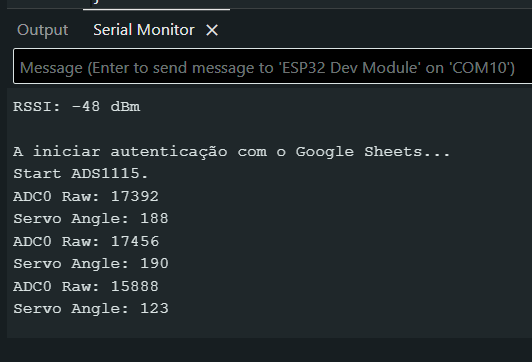
\includegraphics[width=\textwidth]{out1}
		\caption{Monitoramento serial no ESP32}
	\end{minipage}
	\hfill
	\begin{minipage}[b]{0.45\textwidth}
		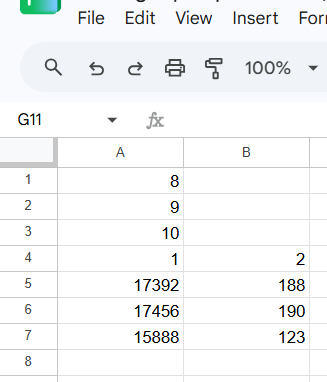
\includegraphics[width=\textwidth]{out2}
		\caption{Dados recebidos pelo Google Sheets}
	\end{minipage}
\end{figure}

\section{Pós-Laboratório}

\subsection{Benefício de empregar um ADC externo quando o sistema contém um ESP32}
Embora o ESP32 possua conversores analógico-digitais (ADCs) internos, o uso de um componente externo como o ADS1115 traz vantagens importantes:
\begin{enumerate}
    \item \textbf{Evita conflitos com o Wi-Fi:} O segundo conversor interno do ESP32 compartilha recursos com o rádio Wi-Fi, o que pode gerar instabilidades ou bloqueios nas leituras durante o uso da rede sem fio. O ADS1115 utiliza comunicação digital ($I^2C$), operando de forma independente do Wi-Fi.
    \item \textbf{Maior precisão e linearidade:} O conversor interno do ESP32 apresenta pequenas limitações e variações de leitura em faixas muito baixas ou muito altas de tensão. O ADS1115 oferece leituras mais estáveis, lineares e confiáveis.
    \item \textbf{Maior resolução:} O ADS1115 possui resolução de 16 bits, o que permite capturar variações de sinal muito mais sutis do que os 12 bits nativos do ESP32.
\end{enumerate}

\subsection{Tipo de ADC empregado no ADS1115 e seu funcionamento}
O ADS1115 utiliza um conversor do tipo \textbf{Delta-Sigma ($\Delta\Sigma$)}. 

Ele funciona amostrando o sinal de entrada em uma frequência muito alta (processo conhecido como sobreamostragem) e convertendo-o em um fluxo rápido de bits. Em seguida, um filtro digital interno processa esse fluxo de dados, eliminando os ruídos de alta frequência e gerando uma leitura digital final de alta precisão e resolução na saída.

\section{Anexos}
\begin{itemize}
    \item Arquivo \texttt{.ino} contendo o código-fonte desenvolvido na Arduino IDE.
\end{itemize}

\end{document}